\documentclass[journal]{IEEEtran}

\usepackage{cite}
\usepackage{amsmath,amssymb}
\usepackage{graphicx}
\usepackage{booktabs}
\usepackage{siunitx}
\usepackage{url}

\graphicspath{{./}{../results/phase3/pure_oai_retry_4way_20260410_144410/plots/}{../../doc/figures/}}
\sisetup{round-mode=places,round-precision=3}

\title{SLA-Aware DRL-Enhanced O-RAN Slice Allocation in a Pure OAI Testbed: A Comparative Study}

\author{Author~One,~\IEEEmembership{Member,~IEEE,}
        Author~Two,~\IEEEmembership{Member,~IEEE,}
        and~Author~Three,~\IEEEmembership{Senior~Member,~IEEE}%
\thanks{Author details are placeholders and will be replaced in the camera-ready version.}%
}
\markboth{IEEE Journal Draft, April 2026}%
{Author \MakeLowercase{\textit{et al.}}: SLA-Aware DRL-Enhanced O-RAN Slice Allocation}

\begin{document}

\maketitle

\begin{abstract}
This paper presents a deep reinforcement learning (DRL)-enhanced resource allocation workflow for 5G network slicing in a pure OpenAirInterface (OAI) testbed. We evaluate four controllers under a common live setup: a rule-based baseline, Deep Q-Network (DQN), Advantage Actor-Critic (A2C), and a rule-based plus DRL hybrid controller. The experiment is executed with fixed seed and controlled traffic replay in a strict OAI-only deployment (no UERANSIM), using a 3-UE triad profile and live Prometheus-derived state feedback. Results on the selected seed-256 run show that all DRL-enhanced controllers outperform the rule-based baseline in mean reward, while DQN achieves the lowest violations-per-step among all tested controllers. We further analyze weighted SLA debt, weighted SLA satisfaction, slice-wide efficiency, and violation burst behavior to discuss the trade-off between policy aggressiveness and stability. The study provides a reproducible manuscript baseline for IEEE-style reporting and identifies limitations of short-horizon single-seed evaluation that motivate future multi-seed, long-horizon validation.
\end{abstract}

\begin{IEEEkeywords}
O-RAN, OpenAirInterface, network slicing, deep reinforcement learning, DQN, A2C, SLA-aware scheduling.
\end{IEEEkeywords}

\section{Introduction}
Fifth-generation (5G) networks rely on radio access network (RAN) slicing to co-host heterogeneous services such as enhanced Mobile Broadband (eMBB), Ultra-Reliable Low-Latency Communications (URLLC), and massive machine-type communications (mMTC). In practical deployments, traffic dynamics and conflicting service-level agreement (SLA) targets make static or threshold-only resource allocation suboptimal. O-RAN disaggregation and near-real-time control loops create an opportunity for learning-based adaptation in slice-level scheduling \cite{ref_oran_alliance,ref_oran_arch}.

This work targets a deployment-constrained but realistic setting based on OAI and Open5GS components, where policy outputs are translated into \texttt{rrmPolicy} updates for slice ratio control. Instead of presenting only offline simulation behavior, we center the analysis on a pure OAI live pipeline and evaluate how DRL controllers compare against a deterministic rule-based baseline under identical runtime conditions. The control loop is implemented as: telemetry acquisition, policy inference, constrained action decoding, policy JSON writeback, and delayed reward evaluation on the next observed state.

The contribution of this manuscript draft is three-fold:
\begin{itemize}
    \item It documents an IEEE-style, reproducible methodology for pure OAI 4-way controller comparison (rule-based, DQN, A2C, hybrid).
    \item It reports controller-level reward and SLA-violation behavior from a verified seed-256 run with consistent traffic initialization.
    \item It provides an interpretable discussion through profile-weighted SLA and burst-oriented plots, linking metrics to operational behavior.
\end{itemize}

In addition to high-level comparisons, this expanded draft formalizes the MDP and action encoding used in the implementation, provides algorithm-level optimization equations for DQN and A2C policies, and reports explicit run-time constraints from the live configuration (slice budgets, ratio bounds, and deterministic replay protocol).

\section{Problem Statement}
The slice allocator is modeled as a discounted Markov decision process (MDP)
\begin{equation}
\mathcal{M}=\left(\mathcal{S},\mathcal{A},\mathcal{P},\mathcal{R},\gamma\right),
\end{equation}
where $\mathcal{S}$ is the encoded telemetry state space, $\mathcal{A}$ is the constrained ratio-allocation action space, $\mathcal{P}$ captures environment dynamics induced by traffic and scheduler response, $\mathcal{R}$ is the SLA-aware reward, and $\gamma\in(0,1)$ is the discount factor.

Let $\mathcal{I}$ denote the set of active slices, and let each slice $i \in \mathcal{I}$ have observed metrics at time step $t$: offered load $o_i(t)$, achieved throughput $x_i(t)$, latency $\ell_i(t)$, and packet loss $p_i(t)$. Each slice has SLA budgets $\bar{\ell}_i$ (latency) and $\bar{p}_i$ (loss). The normalized per-slice feature triplet is
\begin{equation}
\mathbf{z}_i(t)=\left[e_i(t),\lambda_i(t),\phi_i(t)\right],
\end{equation}
with
\begin{equation}
e_i(t)=\min\left(\frac{x_i(t)}{\max(o_i(t),1)},1\right),
\end{equation}
\begin{equation}
\lambda_i(t)=\mathrm{clip}\left(\frac{\ell_i(t)}{\bar{\ell}_i},0,2\right),\;
\phi_i(t)=\mathrm{clip}\left(\frac{p_i(t)}{\bar{p}_i},0,2\right).
\end{equation}
For $|\mathcal{I}|=3$ slices, the state vector is
\begin{equation}
\mathbf{s}(t)=\left[\mathbf{z}_{1}(t),\mathbf{z}_{2}(t),\mathbf{z}_{3}(t)\right]\in\mathbb{R}^{9}.
\end{equation}

The control action at each step is a set of slice-level ratio bounds:
\begin{equation}
\mathbf{a}(t)=\{(\rho^{\min}_i(t),\rho^{\max}_i(t))\}_{i\in\mathcal{I}},
\end{equation}
subject to valid scheduler constraints and policy encoding rules.

Implementation uses a factorized multi-discrete action representation. For each slice, \(\rho^{\min}\) and \(\rho^{\max}\) are each discretized into 12 bins, resulting in
\begin{equation}
|\mathcal{A}_i|=12\times 12=144
\end{equation}
branch actions per slice. The full joint action cardinality is
\begin{equation}
|\mathcal{A}|=\prod_{i\in\mathcal{I}}|\mathcal{A}_i|=144^3=2{,}985{,}984,
\end{equation}
but policy inference is performed branch-wise, then combined by deterministic decoding and bound clipping.

The optimization objective is to maximize long-term utility while minimizing SLA violations:
\begin{equation}
\max_{\pi}\; \mathbb{E}_{\pi}\left[\sum_{t=0}^{T-1} \gamma^t r(t)\right],
\end{equation}
where $\pi$ is the controller policy and $r(t)$ is a per-step reward combining efficiency gain and weighted SLA penalties.

In the implemented framework, reward is computed as:
\begin{equation}
 r(t)=\sum_{i\in\mathcal{I}}\min\left(\frac{x_i(t)}{\max(o_i(t),1)},1\right)
 -\sum_{i\in\mathcal{I}} w_i\left(2\,\delta^{\ell}_i(t)+3\,\delta^{p}_i(t)\right),
\end{equation}
with normalized SLA exceedances
\begin{equation}
\delta^{\ell}_i(t)=\max\left(0,\frac{\ell_i(t)-\bar{\ell}_i}{\max(\bar{\ell}_i,\epsilon)}\right), \quad
\delta^{p}_i(t)=\max\left(0,\frac{p_i(t)-\bar{p}_i}{\max(\bar{p}_i,\epsilon)}\right),
\end{equation}
and profile-dependent priority weights $w_i$ (URLLC $>$ eMBB $>$ mMTC).

Per-step SLA violations are counted as
\begin{equation}
v(t)=\sum_{i\in\mathcal{I}}\mathbb{1}\{\delta^{\ell}_i(t)>0\;\vee\;\delta^{p}_i(t)>0\},
\end{equation}
which is logged alongside reward to expose penalty-efficiency trade-offs.

\section{Objectives}
The concrete objectives of this study are:
\begin{itemize}
    \item Evaluate whether DRL-based controllers improve reward and SLA behavior over a standard rule-based baseline in a pure OAI testbed.
    \item Compare value-based (DQN), policy-based (A2C), and hybrid control under identical seed, traffic, and horizon settings.
    \item Provide a results narrative suitable for IEEE journal reporting, including quantitative summary and diagnostic figures.
    \item Identify limitations and future evaluation requirements for statistically robust publication claims.
\end{itemize}

\section{Methodology}
\subsection{System Setup}
Experiments are executed in a pure OAI environment with Open5GS core functions and OAI gNB/UE components, explicitly excluding UERANSIM. The runtime pipeline enforces live trace collection mode and restarts traffic profiles per controller to preserve seed-level comparability.

The selected evaluation run uses:
\begin{itemize}
    \item Seed: 256,
    \item Horizon: 18 steps,
    \item Step period: 1 second,
    \item Controllers: rule-based, DQN, A2C, rule-based+DRL hybrid,
    \item Checkpointed DRL inference with explicit hybrid mixing weights.
\end{itemize}

At each step, the runner performs: (1) collect state from Prometheus and local counter fallbacks, (2) infer action with the active controller, (3) write constrained \texttt{rrmPolicy.json}, (4) observe next state, and (5) compute reward and violation statistics. The experiment logger stores action vectors, flattened action index, state vectors, per-slice KPIs, and slice-wide aggregates.

\subsection{Controllers}
\textbf{Rule-based baseline} applies deterministic slice-ratio adaptation from current SLA state. \textbf{DQN} estimates action-value scores over encoded ratio actions and selects high-value actions at inference. \textbf{A2C} uses actor-critic parameterization for policy/value estimation. \textbf{Hybrid control} combines rule-based action priors with DQN and A2C guidance through fixed blending weights.

\subsection{Controller Mechanics and Optimization}
\textbf{Threshold rule-based baseline.} The deployed rule-based baseline is a threshold heuristic driven by served-demand ratio
\begin{equation}
\eta_i(t)=\frac{x_i(t)}{\max(o_i(t),\epsilon)}.
\end{equation}
If \(\eta_i(t)<0.80\), the slice score is increased; if \(\eta_i(t)>0.97\), the score is decreased; otherwise it decays slowly. The normalized scores are converted to ratio shares and clipped to per-slice bounds.

\textbf{DQN.} The Q-network uses a two-layer MLP (128, 128) with ReLU activations and per-branch logits. The training objective follows temporal-difference learning:
\begin{equation}
\mathcal{L}_{\mathrm{DQN}}=\mathbb{E}\left[\left(r_t+\gamma\max_{a'}Q_{\theta^-}(s_{t+1},a')-Q_{\theta}(s_t,a_t)\right)^2\right].
\end{equation}
Gradient norm clipping (max norm 1.0), epsilon-greedy exploration, and periodic target-network synchronization are used in training mode.

\textbf{A2C.} A shared actor-critic network (same 128-128 shared trunk) outputs policy logits and state value:
\begin{equation}
A_t=r_t+\gamma V_{\psi}(s_{t+1})-V_{\psi}(s_t),
\end{equation}
\begin{equation}
\mathcal{L}_{\mathrm{actor}}=-\mathbb{E}[\log \pi_{\phi}(a_t|s_t)A_t],\quad
\mathcal{L}_{\mathrm{critic}}=\mathbb{E}\left[\left(V_{\psi}(s_t)-\hat V_t\right)^2\right],
\end{equation}
\begin{equation}
\mathcal{L}_{\mathrm{A2C}}=\mathcal{L}_{\mathrm{actor}}+0.5\mathcal{L}_{\mathrm{critic}}-0.01\,\mathcal{H}(\pi_{\phi}).
\end{equation}

\textbf{Hybrid.} The hybrid controller computes weighted blending of baseline and DRL proposals per slice bound:
\begin{equation}
\rho^{\bullet}_{i,\mathrm{hyb}}=\mathrm{clip}\left(\mathrm{round}\left(w_b\rho^{\bullet}_{i,\mathrm{base}}+w_d\rho^{\bullet}_{i,\mathrm{dqn}}+w_a\rho^{\bullet}_{i,\mathrm{a2c}}\right)\right),\;
\bullet\in\{\min,\max\}.
\end{equation}
Weights are normalized at runtime to ensure \(w_b+w_d+w_a=1\).

\subsection{Run Configuration}
Table~\ref{tab:slice-config} summarizes the exact slice budgets and ratio constraints from the evaluated live configuration.

\begin{table}[t]
\caption{Slice targets and allocation bounds used in the evaluated run}
\label{tab:slice-config}
\centering
\begin{tabular}{lcccc}
\toprule
Slice & Profile & Latency budget & Loss budget & Ratio bounds \\
\midrule
1-0 & eMBB & 45 ms & 2.0\% & min:[5,60], max:[40,100] \\
1-1 & URLLC & 15 ms & 0.8\% & min:[5,60], max:[40,100] \\
1-2 & mMTC & 65 ms & 3.5\% & min:[5,60], max:[40,100] \\
\bottomrule
\end{tabular}
\end{table}

The evaluated hybrid weights were \(w_b=0.20\), \(w_d=0.45\), and \(w_a=0.35\). All controllers used identical telemetry cadence (1 s) and deterministic traffic re-seeding before each controller run.

\subsection{Evaluation Artifacts}
Controller outputs are logged per step and aggregated into \texttt{comparison\_summary.csv}. The plotting stage derives profile- and slice-level diagnostics, including weighted SLA debt/satisfaction, offered-load traces, slice-wide efficiency, and violation burst CDFs.

The run log schema includes both controller-level and slice-level observables: action summary, branch action vector, flattened action index, state vector, per-slice throughput/offered load/latency/loss, per-slice SLA flags, and aggregate slice-wide metrics. This enables post-hoc audits of both optimization behavior and policy safety constraints.

\section{Results and Discussion}
\subsection{Controller-Level Summary}
Table~\ref{tab:controller-summary} reports the primary quantitative results from the selected pure OAI run. All DRL-enhanced methods outperform the rule-based baseline in mean reward. DQN attains the lowest violations-per-step.

\begin{table}[t]
\caption{Pure OAI 4-way run summary (seed=256, horizon=18)}
\label{tab:controller-summary}
\centering
\begin{tabular}{lcc}
\toprule
Controller & Reward mean & Violations/step mean \\
\midrule
Rule-based & -2.254 & 0.889 \\
DQN & -0.446 & 0.722 \\
A2C & -0.142 & 0.778 \\
Rule-based+DRL hybrid & -1.838 & 0.778 \\
\bottomrule
\end{tabular}
\end{table}

Relative to rule-based, reward gains are approximately +1.808 (DQN), +2.112 (A2C), and +0.416 (hybrid). Violation-rate reductions are 18.75\% (DQN) and 12.5\% (A2C and hybrid).

\begin{table}[t]
\caption{Relative improvement over rule-based baseline}
\label{tab:relative-improvement}
\centering
\begin{tabular}{lcc}
\toprule
Controller & Reward improvement & Violation-rate reduction \\
\midrule
DQN & +80.2\% & 18.75\% \\
A2C & +93.7\% & 12.50\% \\
Rule-based+DRL hybrid & +18.4\% & 12.50\% \\
\bottomrule
\end{tabular}
\end{table}

Although absolute rewards remain negative, this is expected under strict SLA-penalty weighting where penalty terms can dominate under congestion. Therefore, relative reward and violations-per-step are the key comparative indicators.

\subsection{Profile-Weighted SLA Behavior}
Fig.~\ref{fig:debt} and Fig.~\ref{fig:satisfaction} show that DRL controllers generally reduce weighted SLA debt and improve weighted SLA satisfaction over the baseline trajectory, with different temporal dynamics. DQN exhibits earlier debt reduction, while A2C reaches the highest reward in the aggregate table.

\begin{figure}[t]
\centering
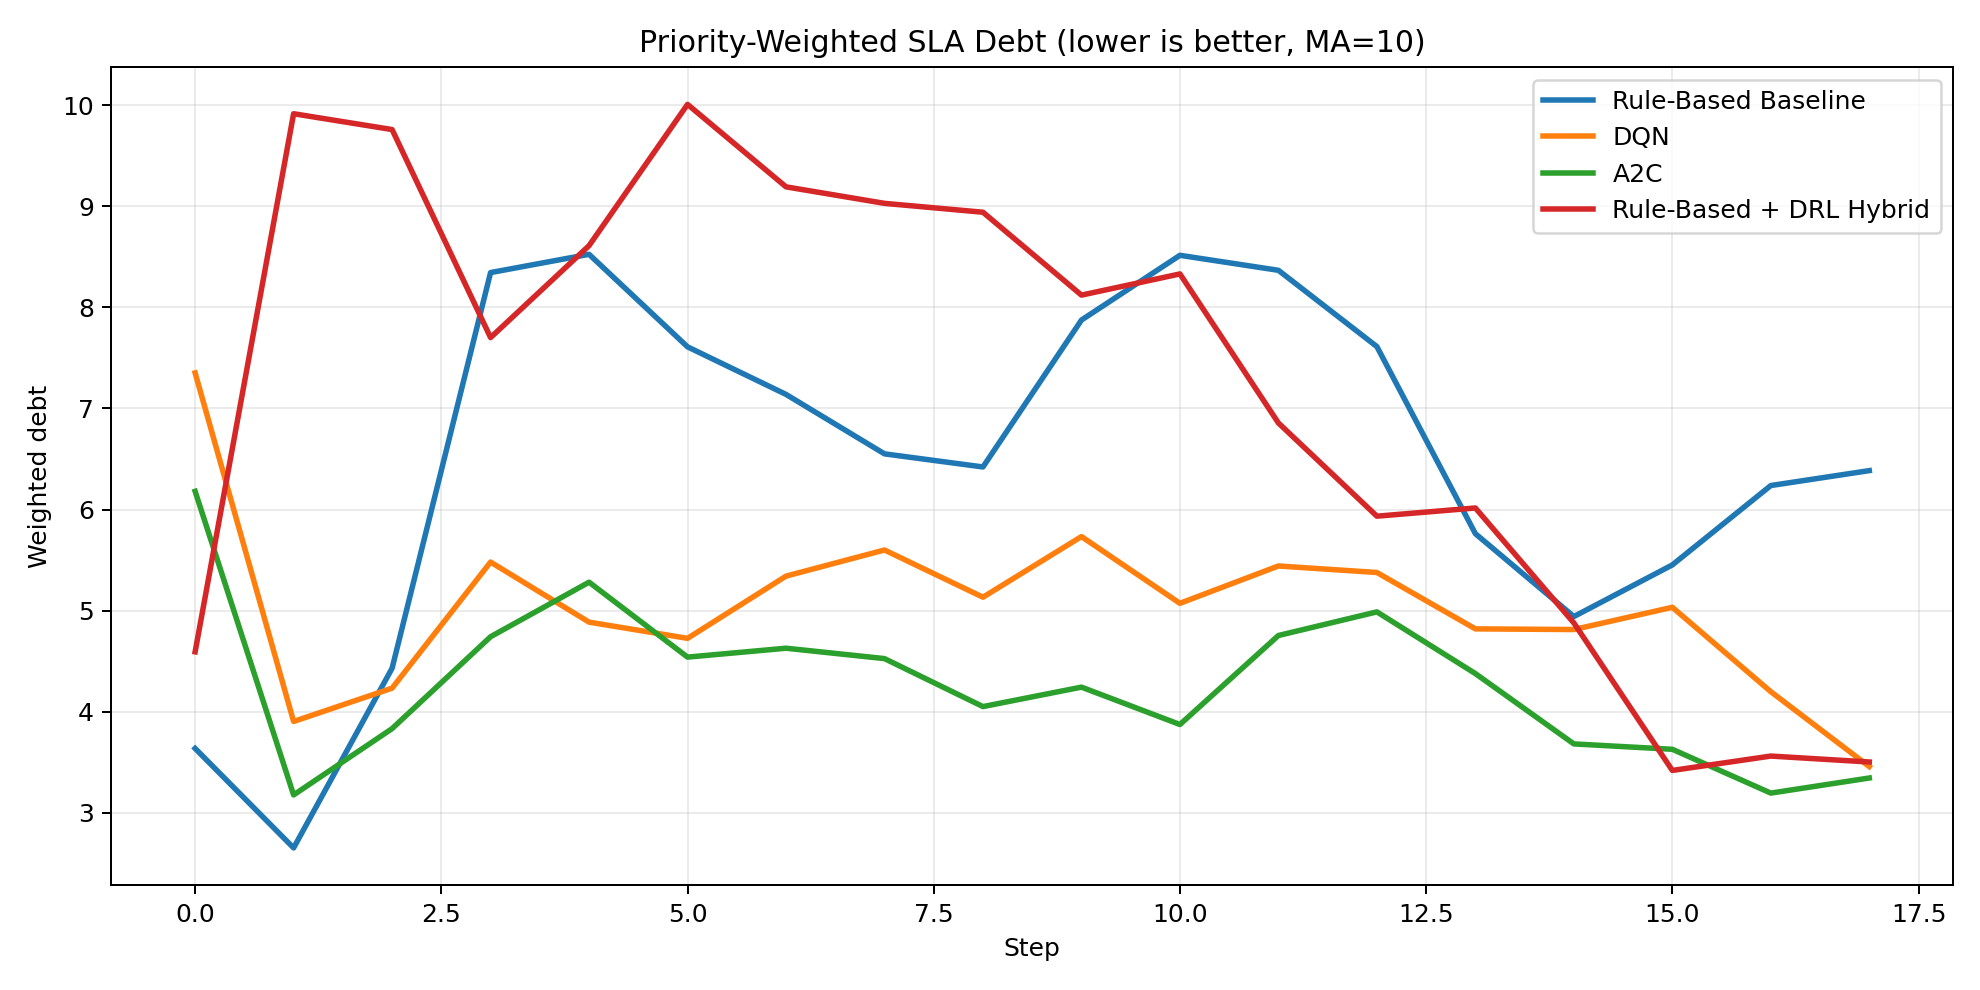
\includegraphics[width=\linewidth]{priority_weighted_sla_debt.png}
\caption{Priority-weighted SLA debt over time (lower is better).}
\label{fig:debt}
\end{figure}

\begin{figure}[t]
\centering
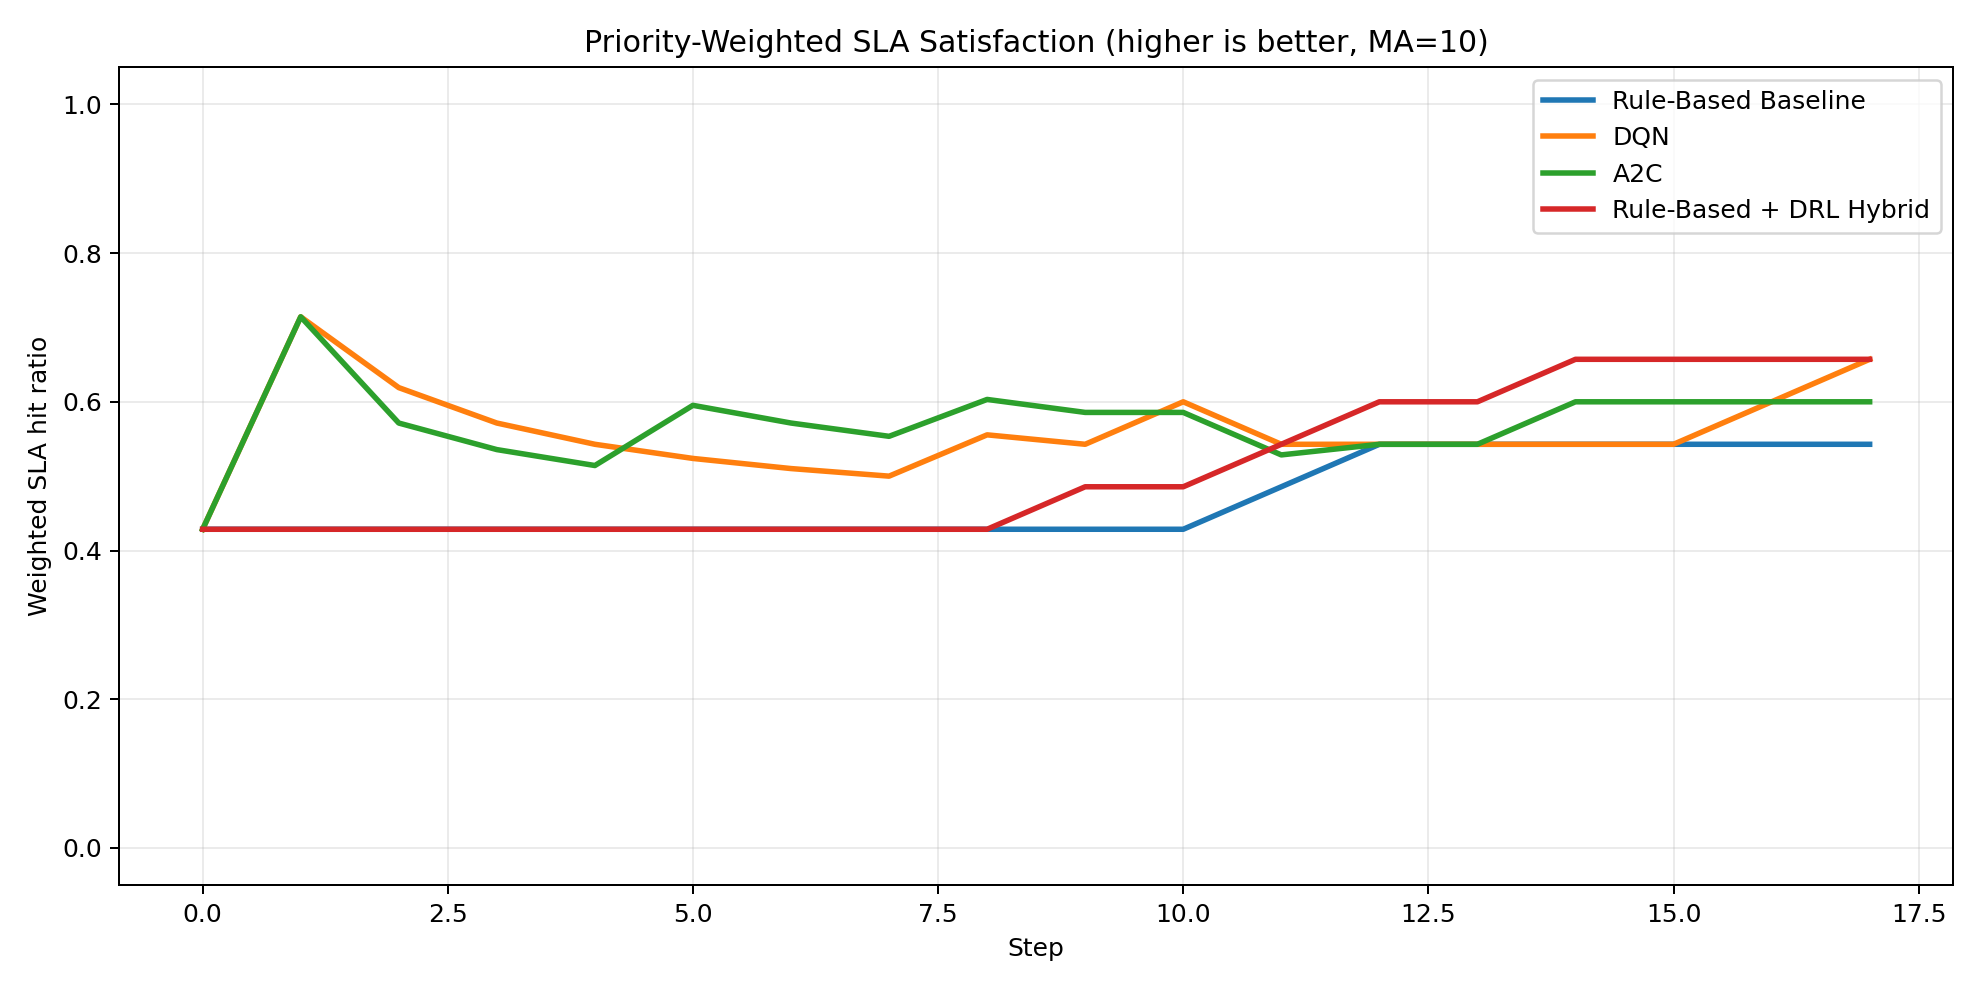
\includegraphics[width=\linewidth]{priority_weighted_sla_satisfaction.png}
\caption{Priority-weighted SLA satisfaction over time (higher is better).}
\label{fig:satisfaction}
\end{figure}

\subsection{Efficiency and Burst Characteristics}
Fig.~\ref{fig:efficiency} indicates that DRL controllers maintain competitive slice-wide throughput efficiency. Fig.~\ref{fig:burstcdf} highlights variation in consecutive violation burst lengths, useful for understanding reliability under transient congestion.

\begin{figure}[t]
\centering
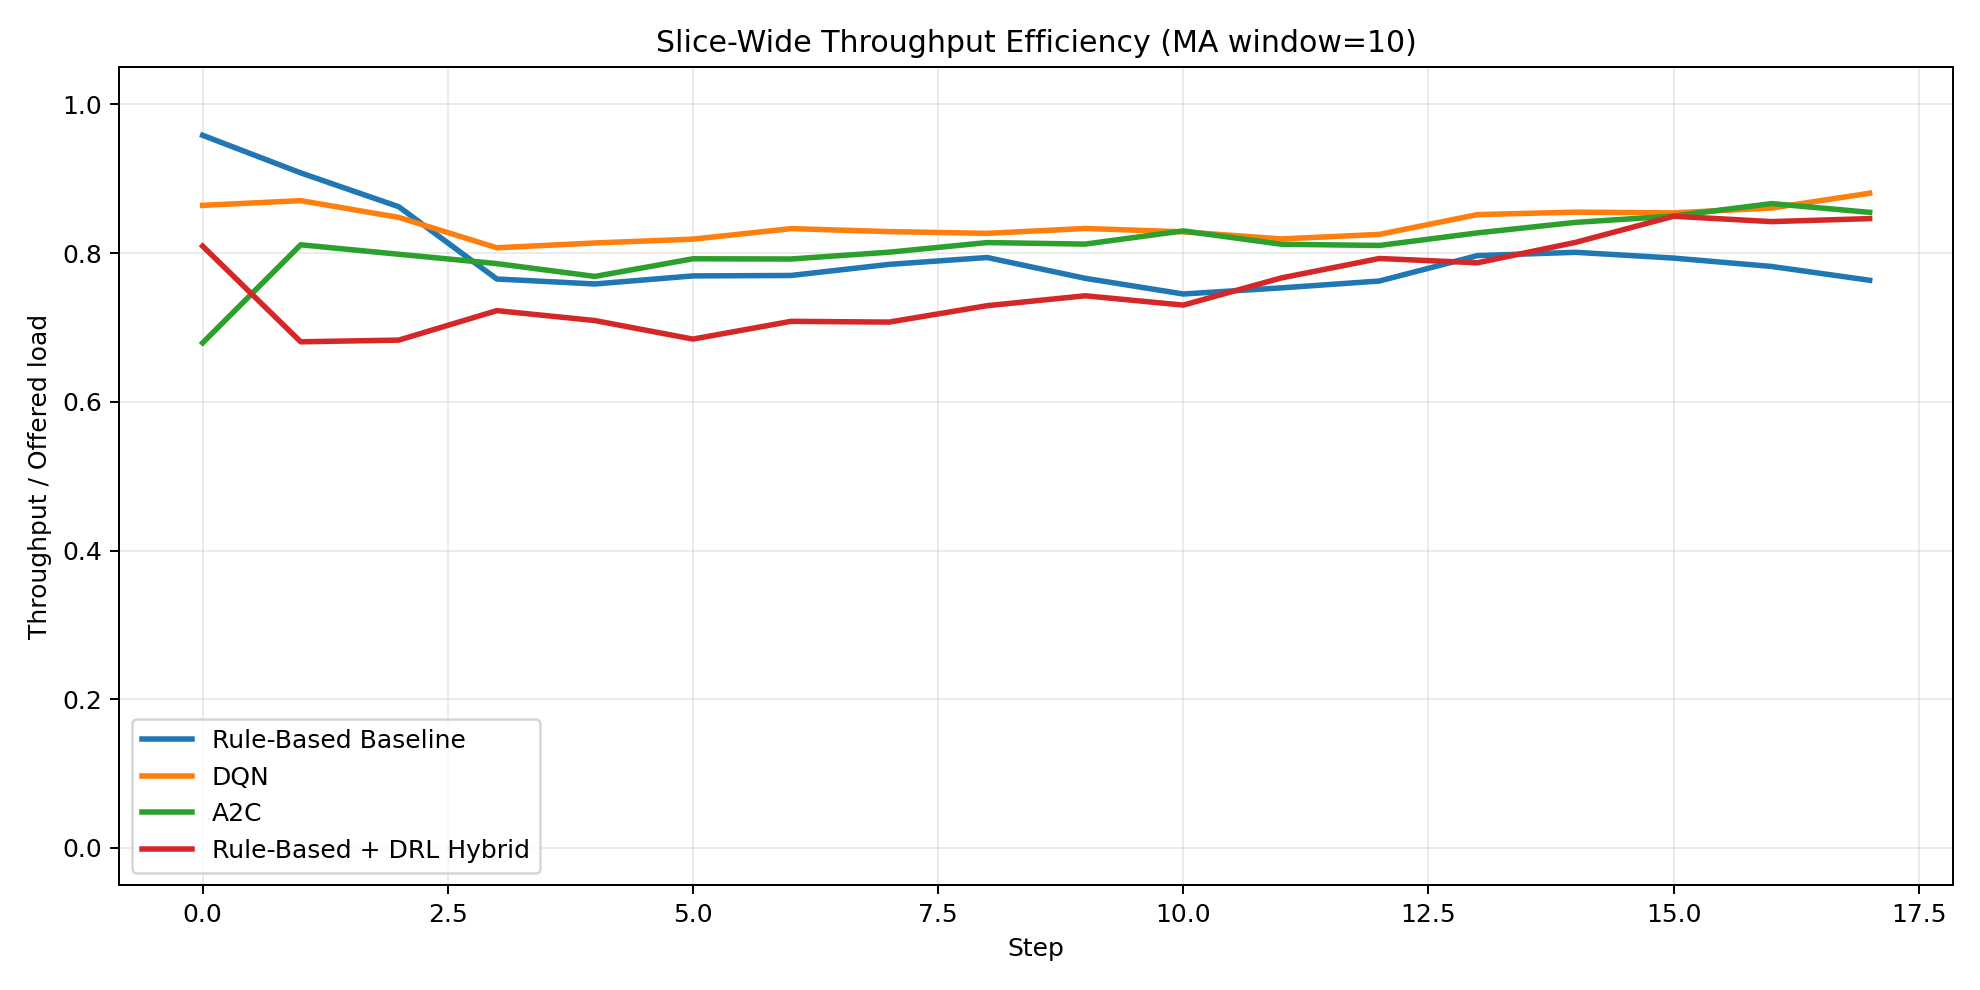
\includegraphics[width=\linewidth]{slice_wide_efficiency.png}
\caption{Slice-wide throughput efficiency trajectory.}
\label{fig:efficiency}
\end{figure}

\begin{figure}[t]
\centering
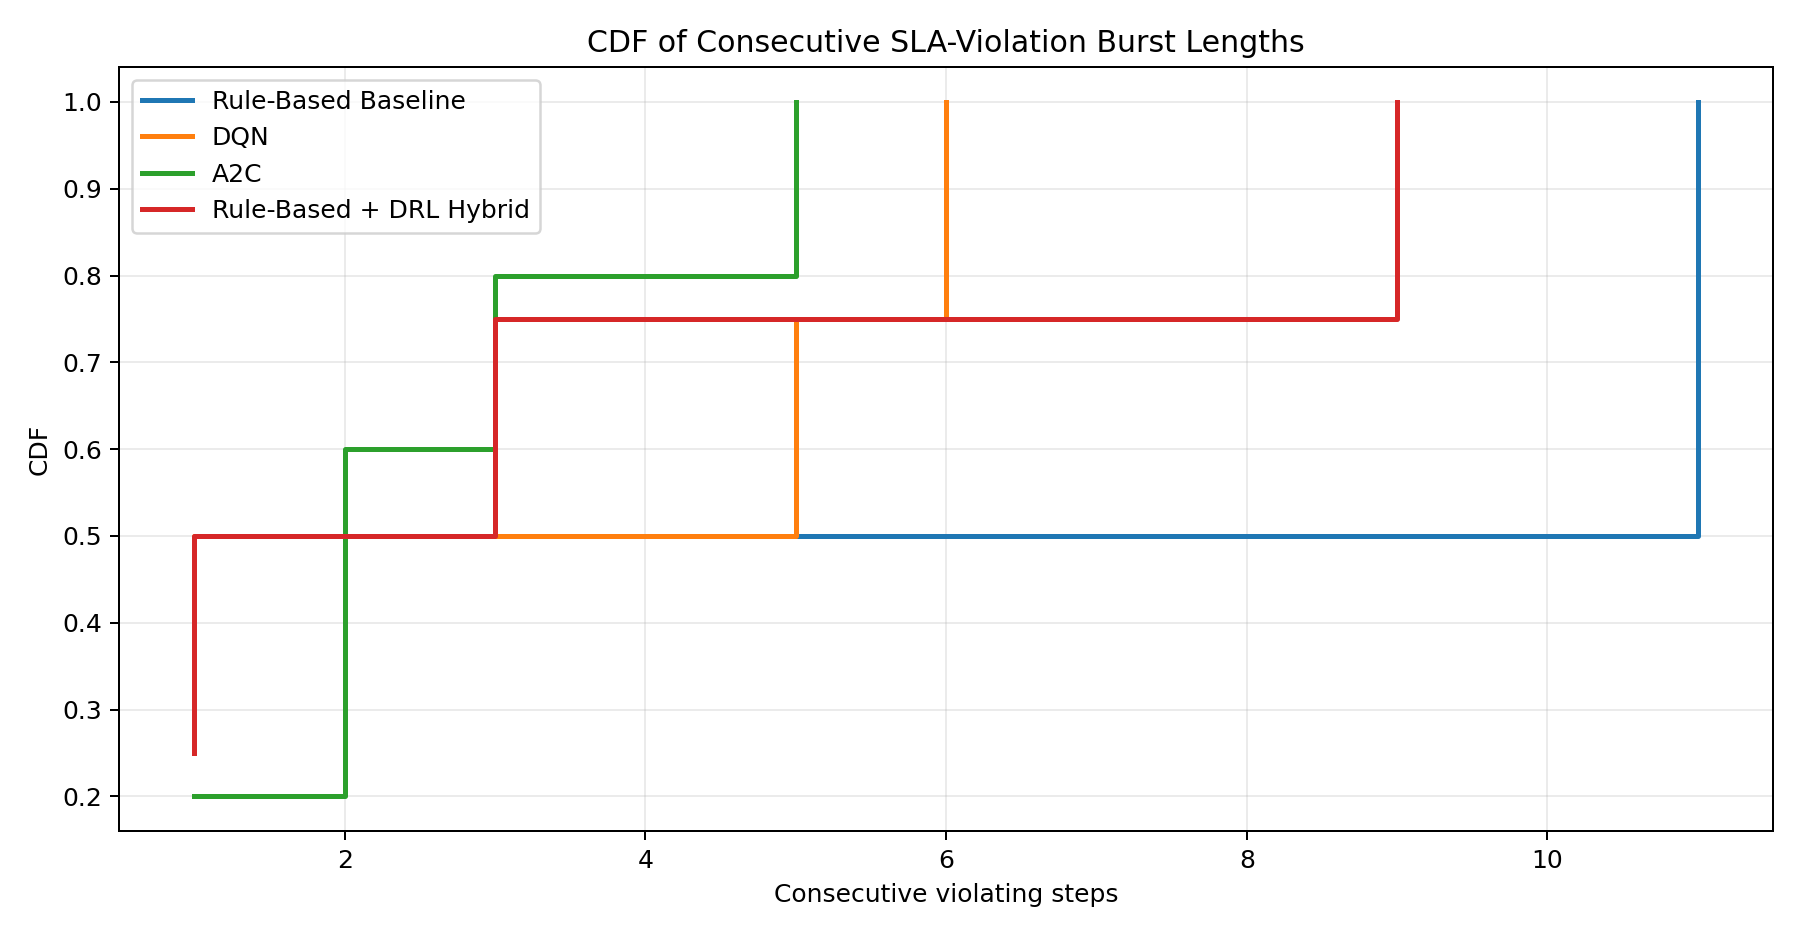
\includegraphics[width=\linewidth]{violation_burst_cdf.png}
\caption{CDF of consecutive SLA-violation burst lengths.}
\label{fig:burstcdf}
\end{figure}

\subsection{Discussion}
The results support the operational hypothesis that DRL-enhanced controllers can improve reward and SLA behavior in an OAI-constrained deployment. DQN shows the strongest violation suppression in this run, while A2C yields the highest reward value, indicating a non-trivial trade-off between strict SLA protection and aggregate utility shaping.

The hybrid controller's moderate gain suggests that weighted blending can stabilize action proposals but may underperform a dominant single learner when weights are not scenario-optimized. This motivates adaptive blending strategies or meta-controllers that reweight baseline/DRL components online.

Methodological limitations remain important. First, this evidence is from a single seed and short horizon, so it is best interpreted as a feasibility signal rather than a final statistical claim. Second, reward sensitivity to profile weights and SLA budgets can alter policy ranking under different traffic stress patterns. Third, policy robustness should be validated under longer congestion episodes, seed sweeps, and richer UE mixes. For publication-grade confidence, future work should expand to multi-seed campaigns, longer horizons, and cross-scenario stress tests \cite{ref_dqn,ref_a2c,ref_5g_slicing}.

\section{Conclusion}
This expanded paper draft documented an implementation-grounded IEEE-style workflow for evaluating DRL-enhanced slice control in a pure OAI testbed. Beyond reporting final metrics, it formalized the MDP, state/action encoding, reward construction, and controller optimization mechanisms used in the codebase. Using a verified seed-256 run, DQN, A2C, and hybrid controllers all exceeded the rule-based baseline in mean reward, while DQN achieved the lowest violations-per-step.

The results and diagnostics indicate that DRL-enhanced policies can improve SLA-aware control quality in a live OAI deployment loop, but robust claims require broader statistical validation. Immediate next steps are: (i) repeat the same protocol across many seeds, (ii) extend horizon and congestion severity, and (iii) evaluate adaptive hybrid weighting. These will convert the current technically sound feasibility result into a fully defensible journal-grade performance study.

\begin{thebibliography}{99}

\bibitem{ref_oran_alliance}
Placeholder, ``O-RAN alliance specification reference,'' to be replaced with final bibliographic entry.

\bibitem{ref_oran_arch}
Placeholder, ``O-RAN architecture and near-real-time RIC reference,'' to be replaced with final bibliographic entry.

\bibitem{ref_dqn}
Placeholder, ``Deep Q-Network foundational reference,'' to be replaced with final bibliographic entry.

\bibitem{ref_a2c}
Placeholder, ``Advantage Actor-Critic foundational reference,'' to be replaced with final bibliographic entry.

\bibitem{ref_5g_slicing}
Placeholder, ``5G slicing optimization and SLA-aware control reference,'' to be replaced with final bibliographic entry.

\end{thebibliography}

\end{document}
